\appendix

\chapter{Unary Operators}
\label{appendix:Unary_Operators}

    
    
    \subsubsection{Logical identity}
        
        Hereafter we have the logical identity operator which we will represent as the function $I(x)$. The logical identity operator takes an argument and returns it as is. 
        
        A logic table for the identity operator has been created and can be found in table \ref{LogicTable:Identity}. In the first column we find our preposition $p$ and its arguments. In the second column we find the return values of the identity operator with the prepositions as the argument $I(p)$.
        
        \begin{table}[h!]
            \centering
            \begin{tabular}{|c|c|}
            	\hline
            	  $p$   & $I(p)$  \\ \hline
            	$true$  & $true$  \\ \hline
            	$false$ & $false$ \\ \hline
            \end{tabular}
            \caption{Logic table of the identity operator where the proposition p, which is either true or false, can be found in the first column. In the second column we find $I(p)$, which is the identity operator with $p$ as its argument, and its return values.}
            \label{LogicTable:Identity}
        \end{table}
        
    \subsubsection{Logical true}
        
        Next we have logical true which we will represent as the function $T(x)$. Logical true takes an argument and always returns true.
        
        A logic table for the true operator has been created and can be found in table \ref{LogicTable:True}. In the first column we find our preposition $p$ and its arguments. In the second column we find the return values of the true operator with the prepositions as the argument $T(p)$.
        
        \begin{table}[h!]
            \centering
            \begin{tabular}{|c|c|}
            	\hline
            	  $p$   & $T(p)$ \\ \hline
            	$true$  & $true$ \\ \hline
            	$false$ & $true$ \\ \hline
            \end{tabular}
            \caption{Logic table of the true operator where the proposition p, which is either true or false, can be found in the first column. In the second column we find $T(p)$, which is the true operator with $p$ as its argument, and its return values.}
            \label{LogicTable:True}
        \end{table}
    
    \subsubsection{Logical false}
        
        Lastly we have logical false which we will represent as the function $F(x)$. Logical false takes an argument and always return false.
        
        A logic table for the false operator has been created and can be found in table \ref{LogicTable:False}. In the first column we find our preposition $p$ and its arguments. In the second column we find the return values of the false operator with the prepositions as the argument $F(p)$.
        
        \begin{table}[h!]
            \centering
            \begin{tabular}{|c|c|}
            	\hline
            	  $p$   & $F(p)$  \\ \hline
            	$true$  & $false$ \\ \hline
            	$false$ & $false$ \\ \hline
            \end{tabular}
            \caption{Logic table of the false operator where the proposition p, which is either true or false, can be found in the first column. In the second column we find $F(p)$, which is the false operator with $p$ as its argument, and its return values.}
            \label{LogicTable:False}
    \end{table}

\chapter{Binary Operators}
\label{appendix:Binaray_Operators}
    \subsubsection{Joint denial}
        Joint denial is represented by $\downarrow$ in mathematics or NOR in computer science and commonly referred to as the NOR operator. The NOR operator results in a true value only if both operands are false.
        
        Using table \ref{LogicTable:PossibleOperators} we see that the set of outputs which corresponds to this definition is column 15 and is summarized in table \ref{LogicTable:NOR}.
        
        Here we have the propositions $p$ and $q$ in the first two columns and all possible permutations between them in the following rows. The last column then shows the resulting value after doing the NOR operation between $p$ and $q$.
        
        \begin{table}[h!]
            \centering
            \begin{tabular}{|c|c|c|}
            	\hline
            	  $p$   &   $q$   & $p \downarrow q$ \\ \hline
            	$true$  & $true$  &     $false$      \\ \hline
            	$true$  & $false$ &     $false$      \\ \hline
            	$false$ & $true$  &     $false$      \\ \hline
            	$false$ & $false$ &      $true$      \\ \hline
            \end{tabular}
            \caption{Logic table of the NOR operator where $p$ is the first proposition and $q$ is the second. All possible permutations are then specified in each row for each proposition. The third column then shows the resulting value of the NOR operation between $p$ and $q$.}
            \label{LogicTable:NOR}
        \end{table}
        
        In disjunctive normal form the NOR operator can be expressed in the following form
        \begin{equation}
            p \downarrow q = (\neg p \wedge \neg q)
        \end{equation}
        using the procedure mentioned in chapter \ref{section:Boolean_algebra}.
    
    \subsubsection{Alternative denial}
        Alternative denial is represented by $\uparrow$ in mathematics or NAND in computer science and commonly referred to as the NAND operator. The NAND operator results in a true value only if one or more of the operands are false.
        
        Using table \ref{LogicTable:PossibleOperators} we see that the set of outputs which corresponds to this definition is column 5 and is summarized in table \ref{LogicTable:NAND}.
        
        Here we have the propositions $p$ and $q$ in the first two columns and all possible permutations between them in the following rows. The last column then shows the resulting value after doing the NAND operation between $p$ and $q$.
        
        \begin{table}[h!]
            \centering
            \begin{tabular}{|c|c|c|}
            	\hline
            	  $p$   &   $q$   & $p \uparrow q$ \\ \hline
            	$true$  & $true$  &    $false$     \\ \hline
            	$true$  & $false$ &     $true$     \\ \hline
            	$false$ & $true$  &     $true$     \\ \hline
            	$false$ & $false$ &     $true$     \\ \hline
            \end{tabular}
            \caption{Logic table of the NAND operator where $p$ is the first proposition and $q$ is the second. All possible permutations are then specified in each row for each proposition. The third column then shows the resulting value of the NAND operation between $p$ and $q$.}
            \label{LogicTable:NAND}
        \end{table}
        
        In disjunctive normal form the NAND operator can be expressed in the following form
        \begin{equation}
            p \uparrow q = (p \wedge \neg q) \vee (\neg p \wedge q) \vee (\neg p \wedge \neg q)
        \end{equation}
        using the procedure mentioned in chapter \ref{section:Boolean_algebra}.
    
    \subsubsection{Logical biconditional}
        The logical biconditional is represented by $\leftrightarrow$ in mathematics or XNOR in computer science and commonly referred to as the exclusive NOR operator. The XNOR operator results in a true value only if both operands are either true or false.
        
        Using table \ref{LogicTable:PossibleOperators} we see that the set of outputs which corresponds to this definition is column 9 and is summarized in table \ref{LogicTable:XNOR}.
        
        Here we have the propositions $p$ and $q$ in the first two columns and all possible permutations between them in the following rows. The last column then shows the resulting value after doing the XNOR operation between $p$ and $q$.
        
        \begin{table}[h!]
            \centering
            \begin{tabular}{|c|c|c|}
            	\hline
            	  $p$   &   $q$   & $p \leftrightarrow q$ \\ \hline
            	$true$  & $true$  &        $true$         \\ \hline
            	$true$  & $false$ &        $false$        \\ \hline
            	$false$ & $true$  &        $false$        \\ \hline
            	$false$ & $false$ &        $true$         \\ \hline
            \end{tabular}
            \caption{Logic table of the XNOR operator where $p$ is the first proposition and $q$ is the second. All possible permutations are then specified in each row for each proposition. The third column then shows the resulting value of the XNOR operation between $p$ and $q$.}
            \label{LogicTable:XNOR}
        \end{table}
        
        In disjunctive normal form the XNOR operator can be expressed in the following form
        \begin{equation}
            p \leftrightarrow q = (p \wedge  q) \vee (\neg p \wedge \neg q)
        \end{equation}
        using the procedure mentioned in chapter \ref{section:Boolean_algebra}.


    \subsubsection{Tautology}
        The tautology operator is represented by $\top$ in mathematics which always returns a true value.
        
        Using table \ref{LogicTable:PossibleOperators} we see that the set of outputs which corresponds to this definition is column 1 and is summarized in table \ref{LogicTable:tautology}.
        
        Here we have the propositions $p$ and $q$ in the first two columns and all possible permutations between them in the following rows. The last column then shows the resulting value after doing the tautology operation between $p$ and $q$.
        
        \begin{table}[h!]
            \centering
            \begin{tabular}{|c|c|c|}
            	\hline
            	  $p$   &   $q$   & $p \top q$ \\ \hline
            	$true$  & $true$  &   $true$   \\ \hline
            	$true$  & $false$ &   $true$   \\ \hline
            	$false$ & $true$  &   $true$   \\ \hline
            	$false$ & $false$ &   $true$   \\ \hline
            \end{tabular}
            \caption{Logic table of the tautology operator where $p$ is the first proposition and $q$ is the second. All possible permutations are then specified in each row for each proposition. The third column then shows the resulting value of the tautology operation between $p$ and $q$.}
            \label{LogicTable:tautology}
        \end{table}
        
        In disjunctive normal form the tautology operator can be expressed in the following form
        \begin{equation}
            p \top q = (p \wedge q) \vee (p \wedge \neg q) \vee (\neg p \wedge q) \vee (\neg p \wedge \neg q)
        \end{equation}
        using the procedure mentioned in chapter \ref{section:Boolean_algebra}.
    
    \subsubsection{Contradiction}
        The contradiction operator is represented by $\bot$ in mathematics which always returns a false value.
        
        Using table \ref{LogicTable:PossibleOperators} we see that the set of outputs which corresponds to this definition is column 16 and is summarized in table \ref{LogicTable:contradiction}.
        
        Here we have the propositions $p$ and $q$ in the first two columns and all possible permutations between them in the following rows. The last column then shows the resulting value after doing the contradiction operator between $p$ and $q$.
        
        \begin{table}[h!]
            \centering
            \begin{tabular}{|c|c|c|}
            	\hline
            	  $p$   &   $q$   & $p \bot q$ \\ \hline
            	$true$  & $true$  &  $false$   \\ \hline
            	$true$  & $false$ &  $false$   \\ \hline
            	$false$ & $true$  &  $false$   \\ \hline
            	$false$ & $false$ &  $false$   \\ \hline
            \end{tabular}
            \caption{Logic table of the contradiction operator where $p$ is the first proposition and $q$ is the second. All possible permutations are then specified in each row for each proposition. The third column then shows the resulting value of the contradiction operation between $p$ and $q$.}
            \label{LogicTable:contradiction}
        \end{table}
        
        In disjunctive normal form the contradiction operator can be expressed in the following form
        \begin{equation}
            p \bot q = p \wedge \neg p
        \end{equation}
    
    \subsubsection{Proposition P}
        We will define the operator Proposition P which results in a true value only if the first operand p is true.
        
        Using table \ref{LogicTable:PossibleOperators} we see that the set of outputs which corresponds to this definition is column 6 and is summarized in table \ref{LogicTable:P}.
        
        Here we have the propositions $p$ and $q$ in the first two columns and all possible permutations between them in the following rows. The last column then shows the resulting value after doing the proposition P between $p$ and $q$.
        
        \begin{table}[h!]
            \centering
            \begin{tabular}{|c|c|c|}
            	\hline
            	  $p$   &   $q$   & $P(p, q)$ \\ \hline
            	$true$  & $true$  &  $true$   \\ \hline
            	$true$  & $false$ &  $true$   \\ \hline
            	$false$ & $true$  &  $false$  \\ \hline
            	$false$ & $false$ &  $false$  \\ \hline
            \end{tabular}
            \caption{Logic table of the proposition P operator where $p$ is the first proposition and $q$ is the second. All possible permutations are then specified in each row for each proposition. The third column then shows the resulting value of the proposition P operation between $p$ and $q$.}
            \label{LogicTable:P}
        \end{table}
        
        In disjunctive normal form the proposition P can be expressed in the following form
        \begin{equation}
            P(p, q) = (p \wedge q) \vee (p \wedge \neg q)
        \end{equation}
        using the procedure mentioned in chapter \ref{section:Boolean_algebra}.
    
    \subsubsection{Proposition Q}
        We will define the operator Proposition Q which results in a true value only if the second operand q is true.
        
        Using table \ref{LogicTable:PossibleOperators} we see that the set of outputs which corresponds to this definition is column 10 and is summarized in table \ref{LogicTable:Q}.
        
        Here we have the propositions $p$ and $q$ in the first two columns and all possible permutations between them in the following rows. The last column then shows the resulting value after doing the proposition Q between $p$ and $q$.
        
        \begin{table}[h!]
            \centering
            \begin{tabular}{|c|c|c|}
            	\hline
            	  $p$   &   $q$   & $Q(p, q)$ \\ \hline
            	$true$  & $true$  &  $true$   \\ \hline
            	$true$  & $false$ &  $false$  \\ \hline
            	$false$ & $true$  &  $true$   \\ \hline
            	$false$ & $false$ &  $false$  \\ \hline
            \end{tabular}
            \caption{Logic table of the proposition P operator where $p$ is the first proposition and $q$ is the second. All possible permutations are then specified in each row for each proposition. The third column then shows the resulting value of the proposition P operation between $p$ and $q$.}
            \label{LogicTable:Q}
        \end{table}
        
        In disjunctive normal form the proposition Q can be expressed in the following form
        \begin{equation}
            P(p, q) = (p \wedge q) \vee (\neg p \wedge  q)
        \end{equation}
        using the procedure mentioned in chapter \ref{section:Boolean_algebra}.
    
    \subsubsection{Negated P}
        We will define the operator negated P which results in a true value only if the first operand p is false.
        
        Using table \ref{LogicTable:PossibleOperators} we see that the set of outputs which corresponds to this definition is column 8 and is summarized in table \ref{LogicTable:NOTP}.
        
        Here we have the propositions $p$ and $q$ in the first two columns and all possible permutations between them in the following rows. The last column then shows the resulting value after doing the negated P between $p$ and $q$.
        
        \begin{table}[h!]
            \centering
            \begin{tabular}{|c|c|c|}
            	\hline
            	  $p$   &   $q$   & $\neg P(p, q)$ \\ \hline
            	$true$  & $true$  &    $false$     \\ \hline
            	$true$  & $false$ &    $false$     \\ \hline
            	$false$ & $true$  &     $true$     \\ \hline
            	$false$ & $false$ &     $true$     \\ \hline
            \end{tabular}
            \caption{Logic table of the negated P operator where $p$ is the first proposition and $q$ is the second. All possible permutations are then specified in each row for each proposition. The third column then shows the resulting value of the negated P operation between $p$ and $q$.}
            \label{LogicTable:NOTP}
        \end{table}
        
        In disjunctive normal form the negated P can be expressed in the following form
        \begin{equation}
            \neg P(p, q) = (\neg p \wedge  q) \vee (\neg p \wedge \neg q)
        \end{equation}
        using the procedure mentioned in chapter \ref{section:Boolean_algebra}.
        
    \subsubsection{Negated Q}
        We will define the operator negated Q which results in a true value only if the second operand q is false.
        
        Using table \ref{LogicTable:PossibleOperators} we see that the set of outputs which corresponds to this definition is column 11 and is summarized in table \ref{LogicTable:NOTQ}.
        
        Here we have the propositions $p$ and $q$ in the first two columns and all possible permutations between them in the following rows. The last column then shows the resulting value after doing the negated Q between $p$ and $q$.
        
        \begin{table}[h!]
            \centering
            \begin{tabular}{|c|c|c|}
            	\hline
            	  $p$   &   $q$   & $\neg Q(p, q)$ \\ \hline
            	$true$  & $true$  &    $false$     \\ \hline
            	$true$  & $false$ &     $true$     \\ \hline
            	$false$ & $true$  &    $false$     \\ \hline
            	$false$ & $false$ &     $true$     \\ \hline
            \end{tabular}
            \caption{Logic table of the negated Q operator where $p$ is the first proposition and $q$ is the second. All possible permutations are then specified in each row for each proposition. The third column then shows the resulting value of the negated operation between $p$ and $q$.}
            \label{LogicTable:NOTQ}
        \end{table}
        
        In disjunctive normal form the negated Q can be expressed in the following form
        \begin{equation}
            \neg Q(p, q) = (p \wedge \neg q) \vee (\neg p \wedge \neg q)
        \end{equation}
        using the procedure mentioned in chapter \ref{section:Boolean_algebra}.
        
    \subsubsection{Material implication}
        Material implication is represented by $\rightarrow$ in mathematics. The material implication operator results in a false value only if the first operand p is true and second operand q is false.
        
        Using table \ref{LogicTable:PossibleOperators} we see that the set of outputs which corresponds to this definition is column 4 and is summarized in table \ref{LogicTable:MI}.
        
        Here we have the propositions $p$ and $q$ in the first two columns and all possible permutations between them in the following rows. The last column then shows the resulting value after doing the material implication operation between $p$ and $q$.
        
        \begin{table}[h!]
            \centering
            \begin{tabular}{|c|c|c|}
            	\hline
            	  $p$   &   $q$   & $p \rightarrow q$ \\ \hline
            	$true$  & $true$  &      $true$       \\ \hline
            	$true$  & $false$ &      $false$      \\ \hline
            	$false$ & $true$  &      $true$       \\ \hline
            	$false$ & $false$ &      $true$       \\ \hline
            \end{tabular}
            \caption{Logic table of the material implication operator where $p$ is the first proposition and $q$ is the second. All possible permutations are then specified in each row for each proposition. The third column then shows the resulting value of the material implication operation between $p$ and $q$.}
            \label{LogicTable:MI}
        \end{table}
        
        In disjunctive normal form the material implication operator can be expressed in the following form
        \begin{equation}
            p \rightarrow q = (p \wedge  q) \vee (\neg p \wedge q) \vee (\neg p \wedge \neg q)
        \end{equation}
        using the procedure mentioned in chapter \ref{section:Boolean_algebra}.
    
    
    \subsubsection{Converse implication}
        Converse implication is represented by $\leftarrow$ in mathematics. The converse implication operator results in a false value only if the first operand p is true and the second q is true.
        
        Using table \ref{LogicTable:PossibleOperators} we see that the set of outputs which corresponds to this definition is column 3 and is summarized in table \ref{LogicTable:CI}.
        
        Here we have the propositions $p$ and $q$ in the first two columns and all possible permutations between them in the following rows. The last column then shows the resulting value after doing the converse implication operation between $p$ and $q$.
        
        \begin{table}[h!]
            \centering
            \begin{tabular}{|c|c|c|}
            	\hline
            	  $p$   &   $q$   & $p \leftarrow q$ \\ \hline
            	$true$  & $true$  &      $true$      \\ \hline
            	$true$  & $false$ &      $true$      \\ \hline
            	$false$ & $true$  &     $false$      \\ \hline
            	$false$ & $false$ &      $true$      \\ \hline
            \end{tabular}
            \caption{Logic table of the converse implication operator where $p$ is the first proposition and $q$ is the second. All possible permutations are then specified in each row for each proposition. The third column then shows the resulting value of the converse implication operation between $p$ and $q$.}
            \label{LogicTable:CI}
        \end{table}
        
        In disjunctive normal form the converse implication operator can be expressed in the following form
        \begin{equation}
            p \leftarrow q = (p \wedge  q) \vee (p \wedge \neg q) \vee (\neg p \wedge \neg q)
        \end{equation}
        using the procedure mentioned in chapter \ref{section:Boolean_algebra}.
    
    \subsubsection{Material nonimplication}
        Material nonimplication is represented by $\not\rightarrow$ in mathematics. The material nonimplication operator results in a true value only if the first operand p is true and the second operand q is false.
        
        Using table \ref{LogicTable:PossibleOperators} we see that the set of outputs which corresponds to this definition is column 13 and is summarized in table \ref{LogicTable:MNI}.
        
        Here we have the propositions $p$ and $q$ in the first two columns and all possible permutations between them in the following rows. The last column then shows the resulting value after doing the material nonimplication operation between $p$ and $q$.
        
        \begin{table}[h!]
            \centering
            \begin{tabular}{|c|c|c|}
            	\hline
            	  $p$   &   $q$   & $p \not\rightarrow q$ \\ \hline
            	$true$  & $true$  &        $false$        \\ \hline
            	$true$  & $false$ &        $true$         \\ \hline
            	$false$ & $true$  &        $false$        \\ \hline
            	$false$ & $false$ &        $false$        \\ \hline
            \end{tabular}
            \caption{Logic table of the material nonimplication operator where $p$ is the first proposition and $q$ is the second. All possible permutations are then specified in each row for each proposition. The third column then shows the resulting value of the material nonimplication operation between $p$ and $q$.}
            \label{LogicTable:MNI}
        \end{table}
        
        In disjunctive normal form the material nonimplication operator can be expressed in the following form
        \begin{equation}
            p \rightarrow q = p \wedge \neg q 
        \end{equation}
        using the procedure mentioned in chapter \ref{section:Boolean_algebra}.
    
    \subsubsection{Converse nonimplication}
        Converse nonimplication is represented by $\not\leftarrow$ in mathematics. The converse nonimplication operator results in a true value only if the first operand p is false and the second operand q is true.
        
        Using table \ref{LogicTable:PossibleOperators} we see that the set of outputs which corresponds to this definition is column 14 and is summarized in table \ref{LogicTable:CNI}.
        
        Here we have the propositions $p$ and $q$ in the first two columns and all possible permutations between them in the following rows. The last column then shows the resulting value after doing the converse nonimplication operation between $p$ and $q$.
        
        \begin{table}[h!]
            \centering
            \begin{tabular}{|c|c|c|}
            	\hline
            	  $p$   &   $q$   & $p \not\leftarrow q$ \\ \hline
            	$true$  & $true$  &       $false$        \\ \hline
            	$true$  & $false$ &       $false$        \\ \hline
            	$false$ & $true$  &        $true$        \\ \hline
            	$false$ & $false$ &       $false$        \\ \hline
            \end{tabular}
            \caption{Logic table of the converse nonimplication operator where $p$ is the first proposition and $q$ is the second. All possible permutations are then specified in each row for each proposition. The third column then shows the resulting value of the converse nonimplication operation between $p$ and $q$.}
            \label{LogicTable:CNI}
        \end{table}
        
        In disjunctive normal form the converse nonimplication operator can be expressed in the following form
        \begin{equation}
            p \leftarrow q =\neg p \wedge q
        \end{equation}
        using the procedure mentioned in chapter \ref{section:Boolean_algebra}.
        
        
\chapter{Control Signal values}
\label{appendix:Controlsignalvalues}
    The tables are on the next few pages as they did not fit the page format.

    \begin{figure}[h!]
        \vspace{-3cm}
        
        \hspace*{-2cm}
        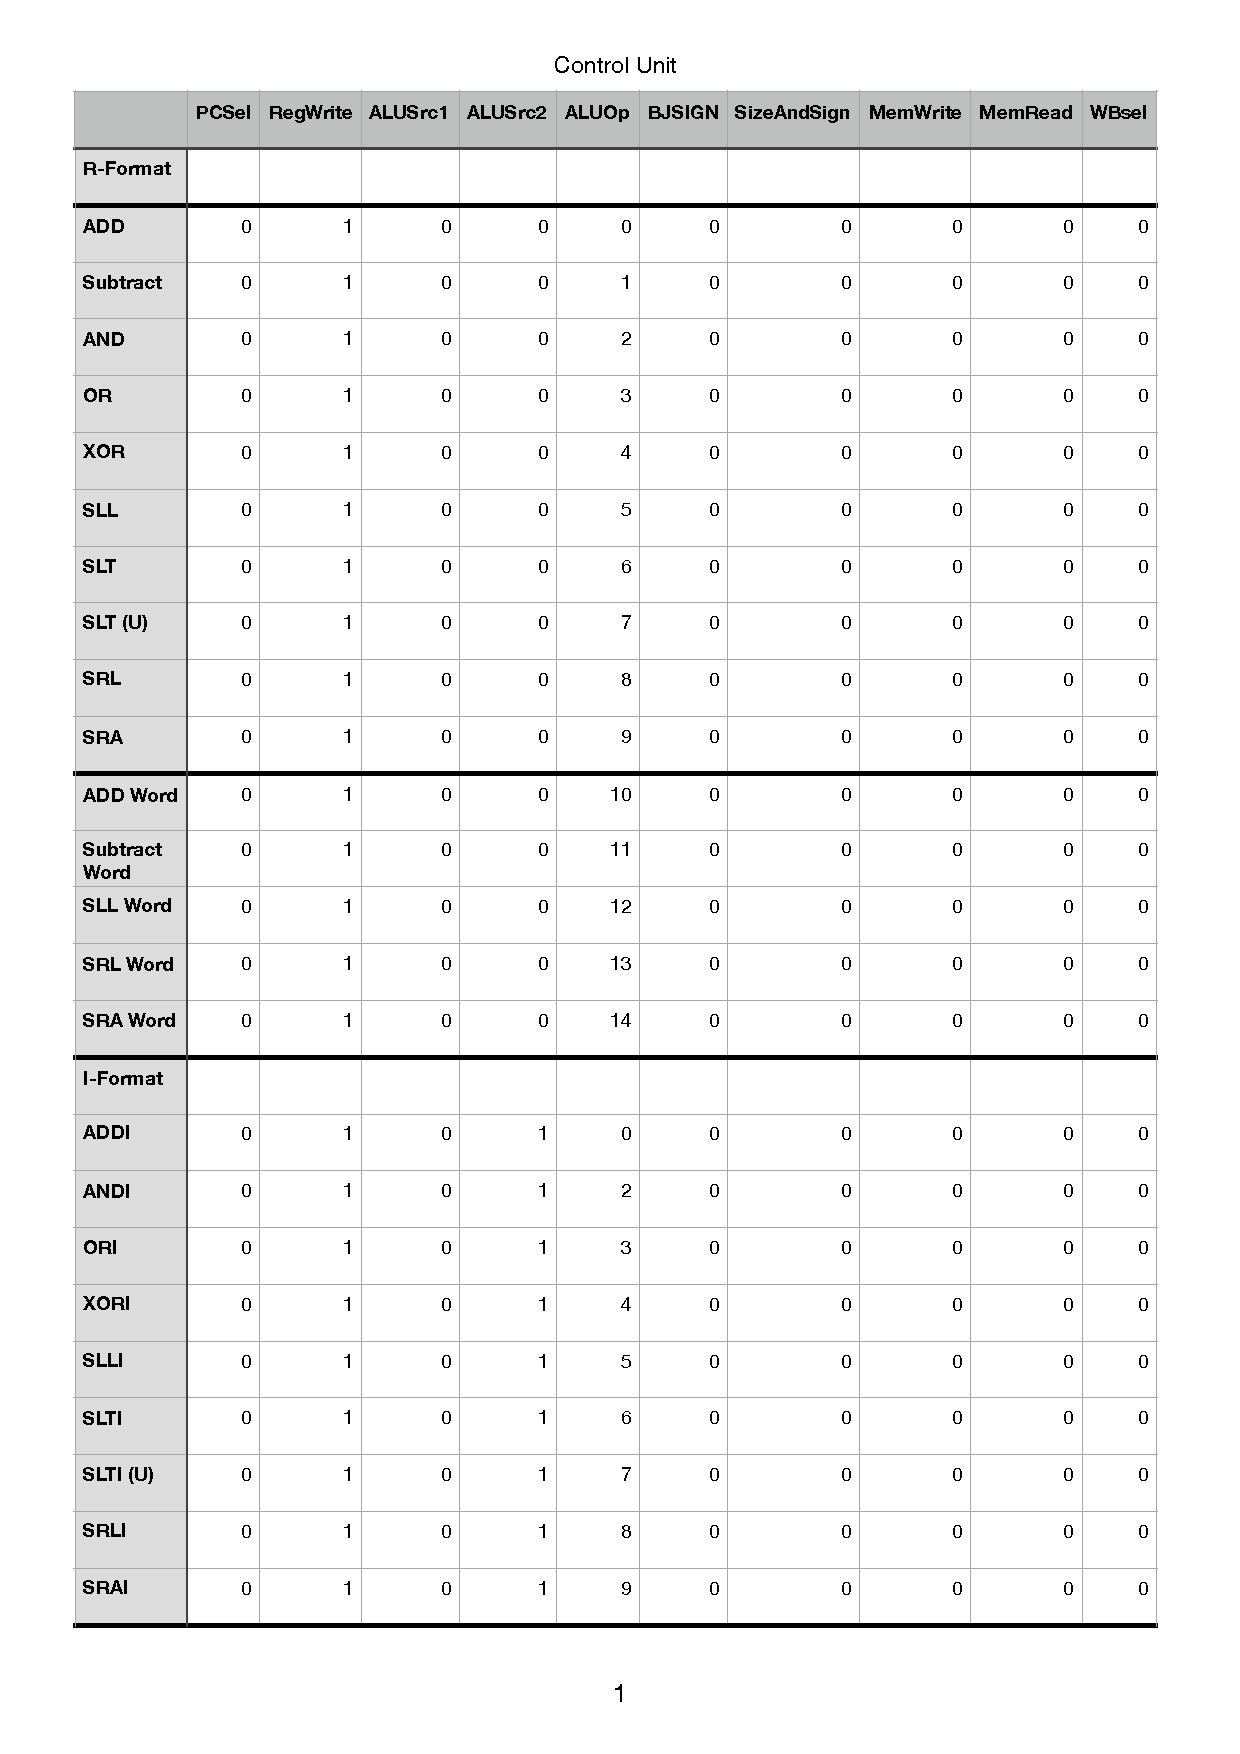
\includegraphics[scale=1]{pictures/Controltable1.pdf}
    \end{figure} 

    \begin{figure}[h!]
        \vspace{-3cm}
        
        \hspace*{-2cm}
        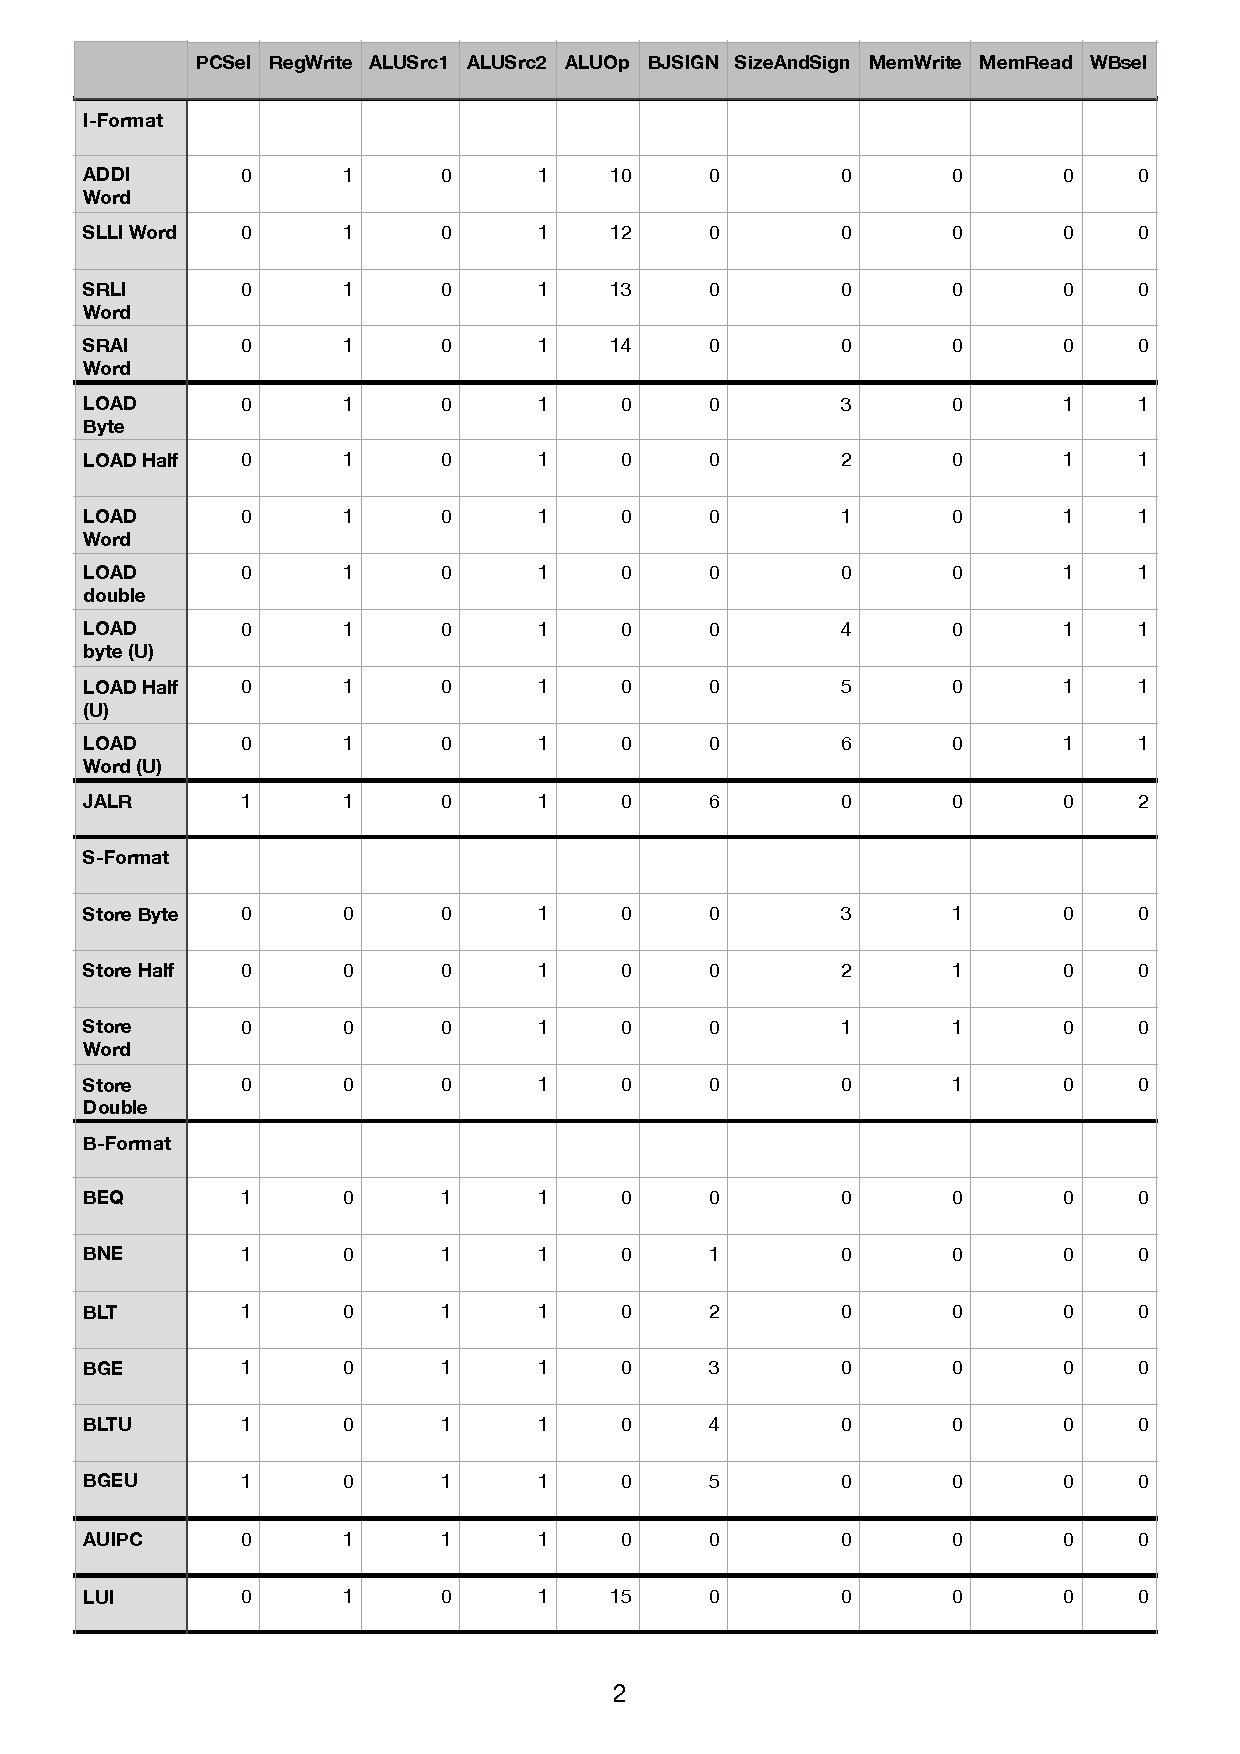
\includegraphics[scale=1]{pictures/Controltable2.pdf}
    \end{figure} 

    \begin{figure}[h!]
        \vspace{-3cm}
        
        \hspace*{-2cm}
        
\includegraphics[scale=1]{pictures/Controltable3.pdf}
    \end{figure} 
